\chapter{Apendice: Cuestionario de Preguntas sobre el Proyecto}

Este apéndice contiene el cuestionario elaborado para el director del proyecto, con el fin de clarificar aspectos técnicos, presupuestales, estructurales y metodológicos relacionados con el desarrollo del kit de clasificación de objetos para el robot PhantomX Pincher.

\section{Requerimientos Generales del Proyecto}

\begin{enumerate}
    \item \textbf{¿La fecha aproximada para la terminación del proyecto es para la semana 8 del semestre 2025-1 o para la semana 8 del semestre 2025-2?}
    
    \item \textbf{¿Cuántos Robot PhantomX Pincher hay en el laboratorio?}
    
    \item \textbf{¿Para cuántos de estos Robots se debe construir el kit?}
    
    \item \textbf{¿Existe un presupuesto para la construcción de cada kit? De ser así, ¿cuál es el presupuesto? (IMPORTANTE)}
\end{enumerate}

\section{Cambios Estructurales y Estética del Robot}

\begin{enumerate}[resume]
    \item \textbf{¿Qué partes actuales del robot se deben o pueden modificar?}
    
    \begin{figure}[H]
    \centering
    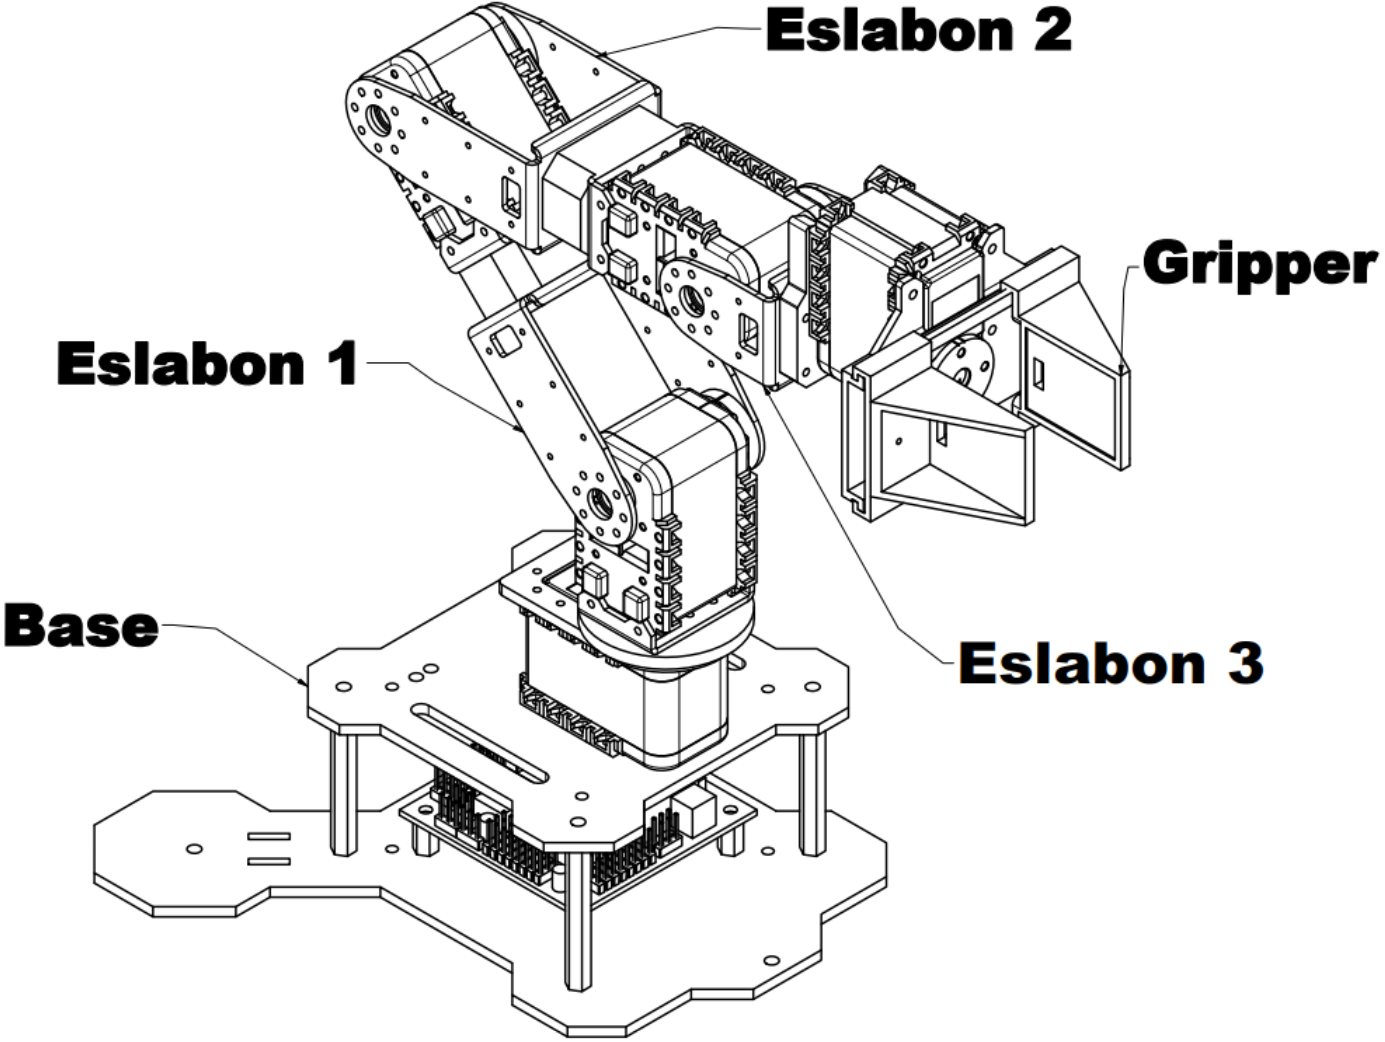
\includegraphics[width=0.6\textwidth]{apendices/img/phantomx_pincher_diagram.png}
    \caption{Diagrama del Robot PhantomX Pincher mostrando sus principales componentes: Base, Eslabón 1, Eslabón 2, Eslabón 3, y Gripper}
    \label{fig:phantomx_diagram}
    \end{figure}
    
    \item \textbf{¿Se desea reemplazar el eslabón 1?}
    
    \textit{Razón de la pregunta: es para saber si se quiere que la estética general del robot se parezca a la del kit de Elephant Robotics}
    
    \item \textbf{¿Se desea reemplazar el eslabón 2?}
    
    \textit{Razón de la pregunta: es para saber si se quiere que la estética general del robot se parezca a la del kit de Elephant Robotics}
    
    \item \textbf{¿Se desea reemplazar el eslabón 3?}
    
    \textit{Razón de la pregunta: es para saber si se quiere que la estética general del robot se parezca a la del kit de Elephant Robotics}
    
    \item \textbf{¿Se puede reemplazar la base del robot?}
    
    \item \textbf{¿Se puede desplazar la electrónica de la base a otra área?}
    
    \item \textbf{¿Se desea tener una copa de succión como en el kit de Elephant Robotics o se puede seguir usando el gripper del Pincher?}
\end{enumerate}

\section{Kit para PhantomX Pincher en Relación con myCobot AI Kit}

\subsection{Estructura de Composición del Sistema en Hardware}

\begin{enumerate}[start=12]
    \item \textbf{Referente a la estructura de composición del sistema del kit en hardware, ¿qué se desea tener de la siguiente lista?}
    
    \begin{itemize}
        \item Brazo mecánico
        \item Base fija
        \item Bomba de succión
        \item Cámara
        \item Módulo identificable
    \end{itemize}
\end{enumerate}

\subsection{Estructura de Composición del Sistema en Software}

\begin{enumerate}[start=13]
    \item \textbf{Referente a la estructura de composición del sistema del kit en software, ¿qué se desea tener de la siguiente lista?}
    
    \begin{itemize}
        \item Módulo de agarre
        \item Módulo de reconocimiento de imágenes
    \end{itemize}
\end{enumerate}

\subsection{Componentes del Kit myCobot AI Kit}

\begin{enumerate}[start=14]
    \item \textbf{Del siguiente listado de componentes del kit que tiene myCobot AI Kit de Elephant Robotics, ¿qué componentes se desea que tenga el kit que se creará?}
    
    \textbf{Componentes del Kit:}
    \begin{enumerate}
        \item Caja de material
        \item Botes de basura
        \item Kit de inteligencia artificial - Placa inferior
        \item Soporte de la caja de material
        \item Cubo (incluye pegatinas)
        \item Bomba de succión
        \item Módulo de visión - Soporte base
        \item Módulo de visión - Cámara
        \item Módulo de visión - Brida de cámara
        \item Módulo de visión - Soporte de cámara
        \item Módulo de visión - Tubo de fibra
        \item Línea de conexión de la bomba de succión - Distribución de energía
        \item Línea de conexión de la bomba de succión - Cable de alimentación
        \item Línea de conexión de la bomba de succión - Cable DuPont
        \item Pantalla LCD
    \end{enumerate}
    
    \begin{figure}[H]
    \centering
    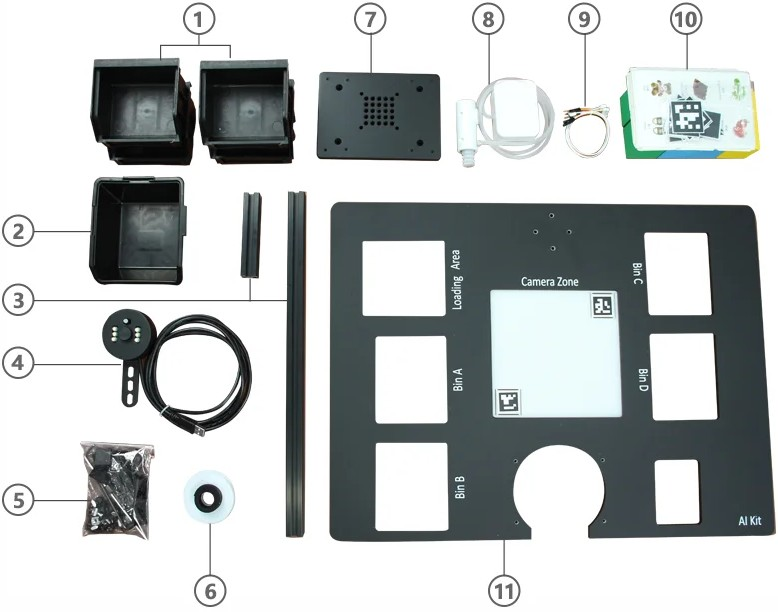
\includegraphics[width=0.8\textwidth]{apendices/img/mycobot_components.jpg}
    \caption{Componentes del myCobot AI Kit de Elephant Robotics}
    \label{fig:mycobot_components}
    \end{figure}
\end{enumerate}

\section{Estructuración de GitHub, Guías y Tutoriales}

\begin{enumerate}[start=15]
    \item \textbf{¿El kit se aplicará en los cursos de Robótica o en qué otros cursos se usarán?}
    
    \item \textbf{¿Se busca que la estructura del GitHub sea similar a las guías que se vieron en el curso de robótica?}
    
    \item \textbf{Si la pregunta anterior fue respondida afirmativamente, ¿qué temáticas se siguieron en las guías pasadas de robótica referente al manejo de ROS? ¿En qué orden?}
    
    \item \textbf{¿Es posible compartir una copia de las guías pasadas de ROS en el curso de Robótica?}
    
    \item \textbf{¿Es posible compartir los repositorios que se hicieron referente al desarrollo de las guías pasadas de ROS 1?}
    
    \item \textbf{De los siguientes temas que se muestran en la página de Elephant Robotics referente a lo que se busca aprender con el kit, ¿cuáles deben aprenderse con las guías?}
    
    \begin{itemize}
        \item ROS
        \item OpenCV
        \item Programación en Python
        \item Principios de control de robot de 6 grados de libertad (6 DOF)
        \item Control del efector final
        \item Visión artificial con IA e inteligencia artificial
        \item Control de pantalla LCD
        \item Detección de sensores inteligentes (color, imagen, código ArUco)
    \end{itemize}
    
    \begin{figure}[H]
    \centering
    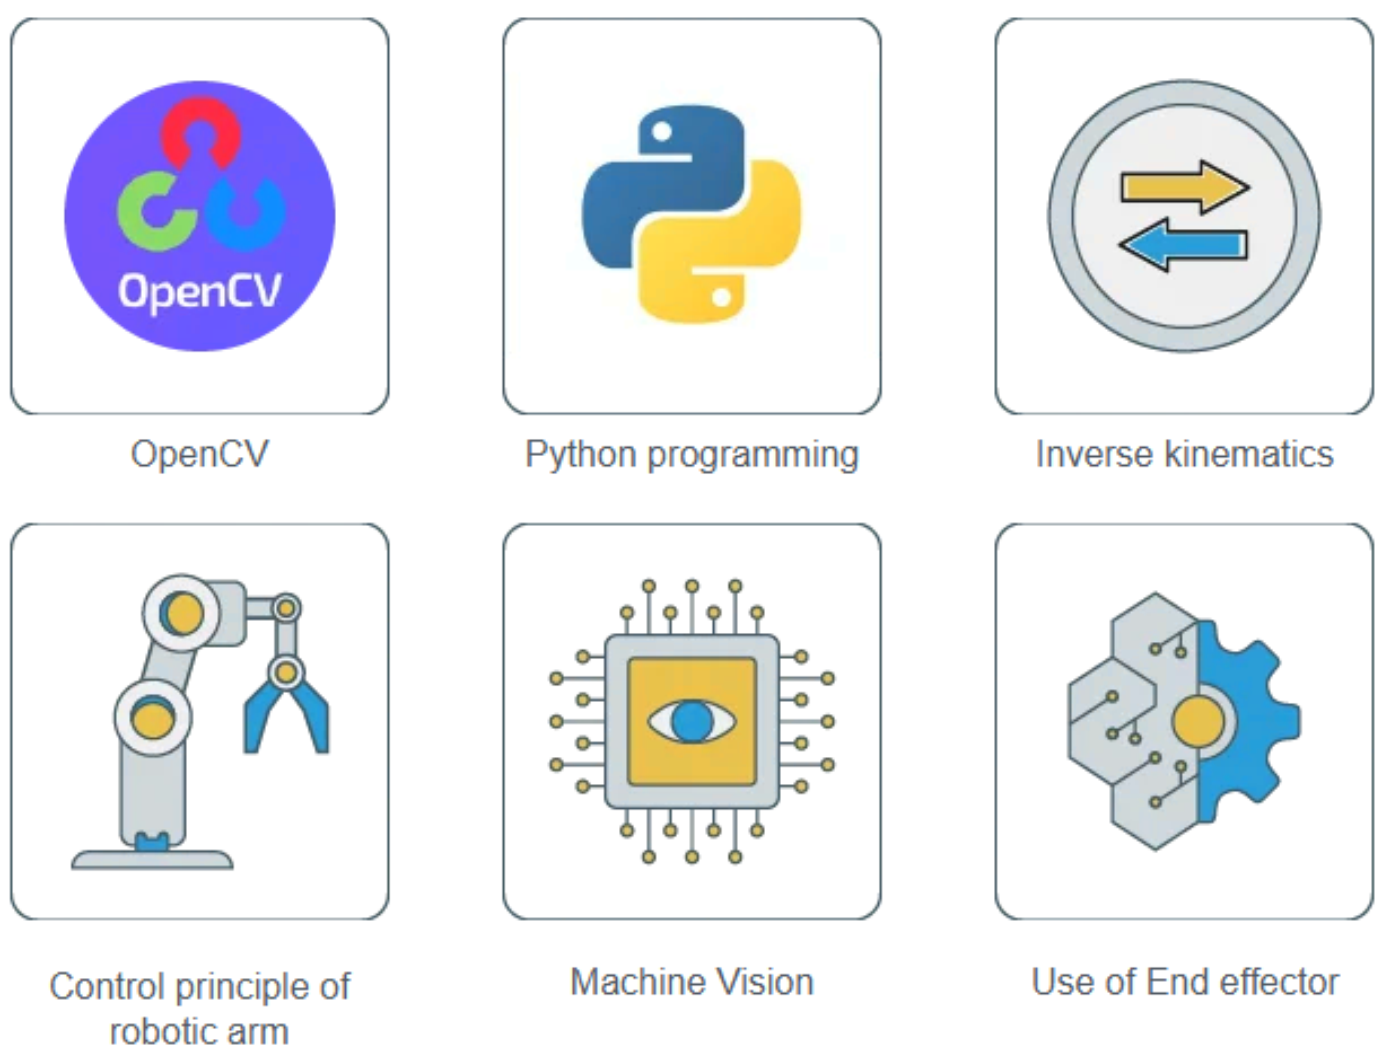
\includegraphics[width=0.9\textwidth]{apendices/img/learning_topics.png}
    \caption{Temas de aprendizaje propuestos por Elephant Robotics: OpenCV, Python programming, Inverse kinematics, Control principle of robotic arm, Machine Vision, y Use of End effector}
    \label{fig:learning_topics}
    \end{figure}
    
    \item \textbf{¿Se puede acompañar con videos y tutoriales las guías que se hagan en GitHub?}
    
    \item \textbf{¿Con cuál cuenta o a qué repositorio de GitHub se debe subir la información del kit y avances del proyecto?}
    
    \item \textbf{De realizarse videos, ¿existen cuentas de YouTube a las cuales se deban subir los videos o se debe crear un canal específico para estos?}
\end{enumerate}

\section{Logística y Organización del Trabajo}

\begin{enumerate}[start=24]
    \item \textbf{¿Cuál es el área de trabajo en la que debo estar para el desarrollo del proyecto (dentro de la universidad en qué laboratorio)? ¿Sería en el laboratorio de automatización?}
    
    \item \textbf{¿Cuáles son los horarios disponibles de los laboratorios para ir a trabajar o avanzar en el desarrollo del proyecto?}
\end{enumerate}


\chapter{Apendice:Respuestas del Director al Cuestionario del Proyecto}

Este apéndice presenta las respuestas proporcionadas por el director del proyecto, Prof. Dr. Ing. Pedro Fabián Cárdenas Herrera, al cuestionario elaborado para definir los requerimientos, alcances y lineamientos del desarrollo del kit de clasificación de objetos para el robot PhantomX Pincher.

\section{Respuestas al Cuestionario}

\begin{enumerate}[label=\arabic*.]
    \item \textbf{¿La fecha aproximada para la terminación del proyecto es para la semana 8 del semestre 2025-1 o para la semana 8 del semestre 2025-2?}
    
    Semestre 2 de 2025.
    
    \item \textbf{¿Cuántos Robot PhantomX Pincher hay en el laboratorio?}
    
    Hay 7 robots en total.
    
    \item \textbf{¿Para cuántos de estos Robots se debe construir el kit?}
    
    Para los 7 robots.
    
    \item \textbf{¿Existe un presupuesto para la construcción de cada kit? De ser así, ¿cuál es el presupuesto?}
    
    Presupuesto máximo de \$600,000 COP por kit, sin contar electrónica.
    
    \item \textbf{¿Qué partes actuales del robot se deben o pueden modificar?}
    
    Se puede modificar la base.
    
    \item \textbf{¿Se desea reemplazar el eslabón 1?}
    
    No se desea reemplazar ningún eslabón.
    
    \item \textbf{¿Se desea reemplazar el eslabón 2?}
    
    No se desea reemplazar ningún eslabón.
    
    \item \textbf{¿Se desea reemplazar el eslabón 3?}
    
    No se desea reemplazar ningún eslabón.
    
    \item \textbf{¿Se puede reemplazar la base del robot?}
    
    Sí, se puede reemplazar la base del robot.
    
    \item \textbf{¿Se puede desplazar la electrónica de la base a otra área?}
    
    Sí, se puede reemplazar la electrónica del robot.
    
    \item \textbf{¿Se desea tener una copa de succión como en el kit de Elephant Robotics o se puede seguir usando el gripper del Pincher?}
    
    Se desea tener una copa de succión.
    
    \item \textbf{Referente a la estructura de composición del sistema del kit en hardware, ¿qué se desea tener?}
    
    Tener cámara.
    
    \item \textbf{Referente a la estructura de composición del sistema del kit en software, ¿qué se desea tener?}
    
    Se desea conservar la pinza. Se desea tener reconocimiento de imágenes.
    
    \item \textbf{Del listado de componentes del kit que tiene myCobot AI Kit de Elephant Robotics, ¿qué componentes se desea que tenga el kit que se creará?}
    
    No se desea tener pantalla LCD.
    
    \item \textbf{¿El kit se aplicará en los cursos de Robótica o en qué otros cursos se usarán?}
    
    Los kits solo se usarán en Robótica.
    
    \item \textbf{¿Se busca que la estructura del GitHub sea similar a las guías que se vieron en el curso de robótica?}
    
    Debe haber un repositorio en GitHub, desde las guías, el diseño y modelo de los kits, así como también un respaldo del sistema operativo de los controladores.
    
    \item \textbf{Si la pregunta anterior fue respondida afirmativamente, ¿qué temáticas se siguieron en las guías pasadas de robótica referente al manejo de ROS? ¿En qué orden?}
    
    Usar de ejemplo las guías anteriores.
    
    \item \textbf{¿Es posible compartir una copia de las guías pasadas de ROS en el curso de Robótica?}
    
    Sí, se pueden ver las guías pasadas de ROS.
    
    \item \textbf{¿Es posible compartir los repositorios que se hicieron referente al desarrollo de las guías pasadas de ROS 1?}
    
    Sí, se pueden ver los desarrollos pasados.
    
    \item \textbf{De los siguientes temas que se muestran en la página de Elephant Robotics referente a lo que se busca aprender con el kit, ¿cuáles deben aprenderse con las guías?}
    
    ROS, OpenCV, Python y Visión de máquina.
    
    \item \textbf{¿Se puede acompañar con videos y tutoriales las guías que se hagan en GitHub?}
    
    Sí, se puede acompañar con videos e imágenes.
    
    \item \textbf{¿Con cuál cuenta o a qué repositorio de GitHub se debe subir la información del kit y avances del proyecto?}
    
    Se usa la organización de LabSIR en GitHub.
    
    \item \textbf{De realizarse videos, ¿existen cuentas de YouTube a las cuales se deban subir los videos o se debe crear un canal específico para estos?}
    
    Sí, a la cuenta de LabSIR en YouTube.
    
    \item \textbf{¿Cuál es el área de trabajo en la que debo estar para el desarrollo del proyecto (dentro de la universidad en qué laboratorio)? ¿Sería en el laboratorio de automatización?}
    
    El área de trabajo es SalaCAM o el Laboratorio de Automatización.
    
    \item \textbf{¿Cuáles son los horarios disponibles de los laboratorios para ir a trabajar o avanzar en el desarrollo del proyecto?}
    
    Horarios a elegir.
\end{enumerate}

